\Chapter{Introduction}
%%%%%%%%%%%%%%%%%%%%%%%%%%%%%%%%%%%%%%%%%%%%%%%%%%%%%%%%%%%%%%%%%%%%%%%%%%%%%%%%%%%%%%%%%%%%
%%%%%%%%%%%%%%%%%%%%%%%%%%%%%%%%%%%%%%%%%%%%%%%%%%%%%%%%%%%%%%%%%%%%%%%%%%%%%%%%%%%%%%%%%%%%
\Section{Motivation} \label{sec:motivation}
%%%%%%%%%%%%%%%%%%%%%%%%%%%%%%%%%%%%%%%%%%%%%%%%%%%%%%%%%%%%%%%%%%%%%%%%%%%%%%%%%%%%%%%%%%%%
%%%%%%%%%%%%%%%%%%%%%%%%%%%%%%%%%%%%%%%%%%%%%%%%%%%%%%%%%%%%%%%%%%%%%%%%%%%%%%%%%%%%%%%%%%%%

A new generation of accelerators dedicated to High Energy Physics
(HEP), would likely be of the TeV scale. Reduction in the size and cost
of such machines is key to their feasibility. 
Investigation into a high gradient candidates for future HEP machines is an active research. 
Traditional accelerating gradients are on the order of 10's of MV/m
with the power source being a klystron gallery.
High gradient structures and schemes such as the 
short pulse, two-beam acceleration (TBA) scheme 
at the Argonne Wakefield Accelerator (AWA) facility
use novel structures to reach 100's of MV/m or more. 
A goal of the AWA group is to demonstrate fully staged TBA, 
achieving a gradient of 250 MV/m. If successful, this would
be the only facility in the world capable of such gradients used for
acceleration of a beam.

TBA requires a drive beam to pass through a decelerating structure and
lose energy through wakefield generation. The electromagnetic wake
is coupled from the decelerator into an accelerating structure, where
the electric field is used to accelerate a second beam. 
This requires two complete and separate beamlines 
operating synchronously with each other.  
The wakefield structures can be metallic or dielectric on either beam line. 
Dielectric structures, having no irises, are simple to manufacture and have demonstrated
high gradient capability at \SI{100}{MV/m} \cite{WeiPaper}. 

The Compact Linear Collider (CLIC) collaboration, proposes a similar TBA scheme with
a \SI{240}{ns} pulse design. This limits the acceleration gradient
to roughly \SI{150}{MV/m} at room temperature due to rf breakdown \cite{CLICdesignReport}.
Higher gradients could be reached when driven by a very short drive
beam pulse, such as the \SI{20}{ns} pulse length proposed by AWA \cite{WeiPaper}. 
While the peak power and gradients are considerably larger in the short pulse scheme, 
the average power is still feasible and within current technology capabilities.
While the two groups vary on approach, they agree that TBA would 
require less infrastructure when constructing a linear TeV scale machine, 
versus the cost of more conventional technology. 

For example, a case study was done comparing the infrastructure 
needed when using traditional \SI{50}{MW} klystron sources.
It would take roughly 35,000 klystrons to construct a linear machine to deliver the same 
\SI{9.2}{TW} power required in the CLIC design specification reports \cite{CLICdesignReport}. 
With TBA, CLIC projected a \SI{3}{TeV} energy at a length of \SI{48}{km}.
In contrast, the Next Linear Collider (NLC) collaboration projected a \SI{1}{TeV} machine 
with length \SI{26}{km}, using X-band klystrons \cite{NLC}. 
This drastic difference occurs in the infrastructure needed to generate and transfer
RF power in the two cases. In TBA, a high charge bunch train is generated in 
a photoinjector and propagated down stream using conventional technology 
(accelerating structures, quads, dipoles, etc). After it has reached the design energy
is focused into specially designed wakefield structures (decelerating structure).
The RF is then generated in the decelerating structure and supplied to the witness 
beam line through a waveguide connection. This has two benefits over traditional klystron technology.
One, you can have structures at higher frequencies (any multiple of the machine frequency), 
which helps push the gradient. Readily available and production klystrons are limited in this aspect.
Second, all the waveguide infrastructure needed to connect a klystron to the accelerating 
structures is eliminated. There is the initial cost near the photoinjector, 
but downstream, much of the infrastructure costs are eliminated.
Theoretically, TBA can deliver the same amount of power as conventional methods with less 
infrastructure, and therefore lower cost, in the case of a large machine. 

Before a detailed understanding of the power and infrastructure trade offs 
can be obtained, the feasibility of staged TBA must be be demonstrated.
Demonstration of staging is especially important, 
as no high energy machine can be built without staging.
Staging is the ability to use two successive accelerating modules to synchronously accelerate 
the same particle bunch. While simple in principle, the difficulties 
in achieving staging should not be underestimated. 
Demonstration of staging proves that a TBA scheme can be scaled to high energies, and whether it is 
feasible to use such methods. Single stage TBA, and staging 
in a simplified scheme have been demonstrated at the AWA in 2016 \cite{tba2017}.
In the simplified scheme, both bunch trains travel through two decelerating stages.
This causes energy loss in stage 1 as the the second bunch train travels to stage 2.
\begin{figure}
	\begin{center}
		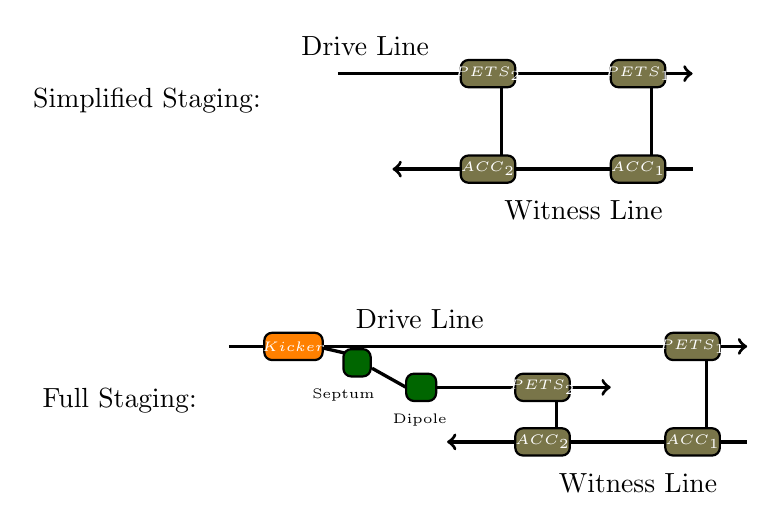
\begin{tikzpicture}[scale=\textwidth/35cm, text=black]
		\def \gunleft {-1.0}
\def \gunright {0.3}
\def \loneright {1.0}
\def \ltworight {2.0}
\def \lthreeright {3.0}
\def \lfourright {4.0}
\def \lfiveright {5.0}
\def \lsixright {6.0}
\def \quadone {7.3}
\def \quadfour{16}

%Full Staging
\draw[very thick, ->] (8,1) -- (27,1);

%Line between kicker and septum
\node[] at (15,2) {Drive Line};
\node[] at (23,-4) {Witness Line};
\draw[very thick] (\lsixright+5.2,1.0) -- (12.5,0.7);

%Kicker 
\draw[fill=orange,  thick, rounded corners =0.1cm] (\lsixright+3.3,0.5)rectangle ({\lsixright+0.84+4.6},1.5) node[pos=.5, white] {\tiny $Kicker$};
%Septum
\node[] at (12.2,-0.8) {\tiny Septum};
\draw[fill=black!60!green,  thick, rounded corners =0.1cm] (12.2,0.9)rectangle ({13.2},-0.1) node[pos=.5, white] {};
%Line between kicker and septum
\draw[very thick] (13.25,0.2) -- (14.5,-0.5);
%Dipole
\node[] at (15,-1.7) {\tiny Dipole};
\draw[fill=black!60!green, thick, rounded corners =0.1cm] (14.5,0.0)rectangle ({15.6},-1.0) node[pos=.5, white] {};
%Line between dipole and quads
\draw[very thick, ->] (15.6,-0.5) -- (22,-0.5);
%Witness
\draw[very thick, <-] (16,-2.5) -- (27,-2.5);
%Waveguide
\draw[very thick] (20,-0.5) -- (20,-3);
%Waveguide
\draw[very thick] (25.5,1.5) -- (25.5,-3);
%PETS2
\draw[fill=black!60!yellow,  thick, rounded corners =0.1cm] (18.5,0.0)rectangle (20.5,-1) node[pos=.5, white] {\tiny$\text{PETS}_2$};
%PETS1
\draw[fill=black!60!yellow,  thick, rounded corners =0.1cm] (24,1.5)rectangle (26,0.5) node[pos=.5, white] {\tiny$\text{PETS}_1$};
%ACC2
\draw[fill=black!60!yellow,  thick, rounded corners =0.1cm] (18.5,-2)rectangle (20.5,-3) node[pos=.5, white] {\tiny$\text{ACC}_2$};
%ACC1
\draw[fill=black!60!yellow,  thick, rounded corners =0.1cm] (24,-2)rectangle (26,-3) node[pos=.5, white] {\tiny$\text{ACC}_1$};



%Simplified Staging



\draw[very thick, ->] (12,11) -- (25,11);

%Line between kicker and septum
\node[] at (13,12) {Drive Line};
\node[] at (21,6) {Witness Line};

%Witness
\draw[very thick, <-] (14,10-2.5) -- (25,10-2.5);
%Waveguide
\draw[very thick] (18,11.5) -- (18,7);
%Waveguide
\draw[very thick] (23.5,11.5) -- (23.5,10-3);
%PETS2
\draw[fill=black!60!yellow,  thick, rounded corners =0.1cm] (16.5,11.5)rectangle (18.5,10.5) node[pos=.5, white] {\tiny$\text{PETS}_2$};
%PETS1
\draw[fill=black!60!yellow,  thick, rounded corners =0.1cm] (22,11.5)rectangle (24,10.5) node[pos=.5, white] {\tiny$\text{PETS}_1$};
%ACC2
\draw[fill=black!60!yellow,  thick, rounded corners =0.1cm] (16.5,8)rectangle (18.5,7) node[pos=.5, white] {\tiny$\text{ACC}_2$};
%ACC1
\draw[fill=black!60!yellow,  thick, rounded corners =0.1cm] (22,8)rectangle (24,7) node[pos=.5, white] {\tiny$\text{ACC}_1$};








		\node[fill=white, inner sep=2pt] (txt2) at (5,10) {Simplified Staging:};
		\node[fill=white, inner sep=2pt] (txt2) at (4,-1) {Full Staging:};
		\end{tikzpicture}
	\end{center}
	\caption{Simplified drawing of the two staging schemes.
		The arrows indicate what direction the beams travels.
		'Simplified staging' refers to experiments that took place at the AWA  prior to 2017.
		'Full Staging' refers to the TBA scheme that is the subject of this thesis.
		Installation efforts are currently ongoing.
		PETS stands for Power Extraction and Transfer Structure, and ACC stands for Accelerating structure. 
		The subscript on each structure refers to which stage the structures belong to (first or second). 
		In the simplified staging scheme the stages are not separated, meaning bunch train two travels
		through and loses energy in the first stage before reaching the second stage.
		This is prevented by separate beam lines in the full staging layout. }
	\label{fig:one}
\end{figure}

Fully staged TBA introduces a fast rise time kicker
and subsequent dogleg-like beam line. In this scenario, bunch trains can be 
be directed to two independent decelerating structures. 
Therefore you can extract the maximum amount of power in each stage.
The thesis work included experimental preparation of fully staged TBA, 
along with beam line design and optimization. 

Chapter 2 details the experimental setup, which included ultraviolet laser pulse train improvement, 
which improves the RF power generation in the wakefield structures.
Also discussed are measurements of the RF power in the gun and linac cavities.
Description of beam size analysis and an image processing script written in Python is covered.
In Chapter 3, the simulation code, OPAL~\cite{opal}, and model used for beam line design is covered in detail.
Benchmarking and initial optimization work is discussed. The photoinjector was optimized for \SI{40}{nC}. 
In Chapter 4, the design of a stripline kicker is discussed. 
The achievable kicker angle and mechanical constraints at the AWA 
were used to lay out the fully staged TBA beam line. 
Simulations of the configuration were done to ensure transmission at
the wakefield structure downstream. Optimization of the optics was done using 
a genetic algorithm and confirm the configuration can transmit a \SI{40}{nC} beam.


%%%%%%%%%%%%%%%%%%%%%%%%%%%%%%%%%%%%%%%%%%%%%%%%%%%%%%%%%%%%%%%%%%%%%%%%%%%%%%%%
\Section{Power Generation}

Wakefields are RF energy that is generated in a structure when a beam passes by. 
The electromagnetic fields
associated with the beam induce surface charges on the structure walls.
If the material has a finite conductivity, discontinuities, or both, the
surface charges will lag behind the beam. These charges then induce
transverse and longitudinal field components in the structure as they
pass irregularities. The resulting electric potential
generated by the beam is commonly called the wake potential, which
is defined as the total voltage lost by a charge following the beam
at some finite distance \cite{SLACwakefields}. The wake potential is 
often calculated numerically using a simulation code. Once calculated, 
the wake potential can then be used to determine how much energy the 
beam will lose after passing through a specific structure. 

Metallic structures used in simplified staging experiments at the AWA, consist of 35 cells and irises. 
The dielectric PETS are also under development at the AWA. 
They consist of a cylindrical metal tube lined with a dielectric \cite{PETSeq}, 
see Fig. \ref{fig:PETS}. Both are candidates for use in full staging, and 
the dielectric structures are especially attractive due to their simplicity. 
The simple geometry reduces cost and complications during fabrication.
It is also easier to damp higher order modes. For example, longitudinal slots in the metal tube surrounding
the dielectric can disrupt the current that supports higher order modes.   
\begin{figure}
	\begin{center}
		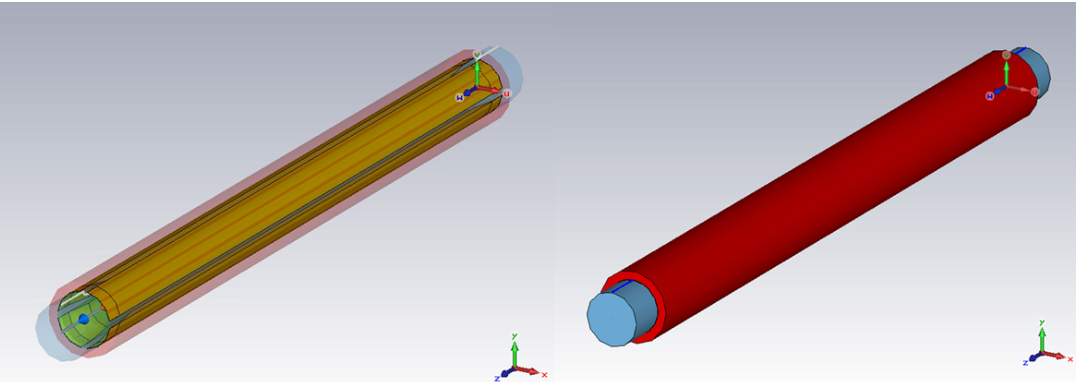
\includegraphics[width=0.8\textwidth]{images/pets-cst.png}
		\caption{CST drawing of a dielectric PETS design, courtesy C. Jing at AWA}
		\label{fig:PETS}
	\end{center}
\end{figure}
In addition to simplicity in fabrication, an analytic solution for the electric fields
in a cylindrical dielectric are still achievable using Maxwell's equations and theory developed
by Rosing and Gai \cite{RosingWei}:
\begin{equation}
E^m_z\left(r,\theta,z_0\right)= \frac{N}{\sigma \sqrt{2\pi}}\int_{-\infty}^{z_0}E^m_0\left(r,\theta,z\right)e^{-\left[\frac{\left(z_0-z\right)^2}{2\sigma^2}\right]}dz
\end{equation}
This form of the electric field is shown to depend 
on the material properties of the structure, and more specifically the permittivity,  $\epsilon$. 
Materials with auspicious permittivities can be chosen to support larger fields
in the longitudinal direction, the field component 
used for acceleration.   
After maximizing the electric field, the wake potential can be calculated: 
\begin{equation}
W_z\left(s\right)= -\frac{1}{eL} \int_{0}^{L} dz E_z \left(z,\frac{\left(z+s\right)}{c}\right)
\label{eq:wakepotential}
\end{equation} 

As shown by the negative sign in equation \ref{eq:wakepotential}, wakefields are a source of 
energy loss in the beam, often disrupting desired particle trajectories, 
and were considered an undesirable side effect.
However, people studying wakefields quickly realized that fields
generated by beams in certain structures resemble fields externally 
applied to cavities or waveguides used to accelerate particle beams.
Hence, the idea to use wakefields as a power source for beam acceleration. 

Note, while wakefield generation is a crucial tool used in TBA at the AWA, the thesis does not include 
structure design. Other members of the AWA group have designed the PETS and accelerating
structures. The thesis will focus on beam line design and beam dynamics. 



\Subsection{Ideal Power Output from Decelerating Structure}
The acceleration gradient achieved at the AWA will depend heavily 
on the PETS and accelerating structure designs, and beam quality 
provided to those structures. This section will focus on the 
structures in use at the AWA and the design specifications of future 
dielectric structures. All PETS and accelerating structures 
used in the simplified staging scheme were metallic. 
While the field is not as high as a dielectric structure would provide,
they have proven to be a great first step 
in determining whether or not TBA was possible at the AWA. Given 
the simplified scheme, predictions can and were made for the acceleration 
gradient and energy gain, based on well known principles. 

A few key equations demonstrate the relationship between beam 
parameters and the resulting power generated in the decelerating structures.  
Starting with the timing, each bunch is separated
in time by $T_{b}=769\,[ps]$, and the average beam current can be written as $I=\frac{Q}{T_{b}}$, 
where $Q$ is the ideal bunch charge.
The bunches are finite and Guassian in the longitudinal direction. Therefore the fields 
generated by the bunch are related to the shape, and do not fill the structure as an
rf pulse from a klystron would.  A form factor, $\Phi$, 
must be calculated to scale the resulting rf power accordingly. 
The form factor, $f(z)$, is calculated 
by taking the Fourier transform of the Guassian charge distribution \cite{PETSeq}: 
\begin{equation}
f\left(z\right) = \frac{q}{\sigma_z \sqrt{2\pi}}exp\left(-\frac{z^2}{2\sigma^2_z}\right)
\end{equation}   
\begin{equation}
\Phi = \left|\frac{1}{q}\int_{-\infty}^{+\infty}f\left(z\right)e^{-jk_z z}z\right|
\end{equation}
\begin{equation}
\Phi=exp\left[\frac{-(k_{z}\sigma_{z})^{2}}{2}\right]
\end{equation}
Where $k_{z}=\frac{2\pi}{\lambda_{z}}$ is the longitudinal wave number
of the decelerating structure, and $\sigma_{z}$ is the rms bunch length \cite{PETSeq}. 
Note the subscript z refers to the characteristics of the structure and bunch in the longitudinal
direction. 

When a Guassian bunch, as described above, travels through a 
decelerating structure, it radiates electromagnetic waves and 
power is lost in the structure. Conservation of energy dictates 
that the amount of power left in the beam 
after it travels some distance through the structure is equal to 
to the total power the beam started with
minus the power lost to the structure through electromagnetic radiation. 
Using this concept, Whittum derived an expression for the power, $P_t$, 
generated by the beam as it travels through a structure \cite{Whittum}. 
\begin{equation}
P_t = \frac{E^2_a}{2 \alpha R}
\label{eq:power1}
\end{equation} 
Where $\alpha=\frac{\omega}{2Q_{d}v_{g}}$ is the attenuation constant of the 
decelerating structure \cite{CLICdesignReport, Whittum}, which quantifies 
how much power in the bunch is transferred into usable electric field. R is the shunt impedance
per unit length, and $E_a$ is the longitudinal electric field in the structure
generated by the beam. 
$E_a$ can be written with respect to 
the structure parameters and beam current \cite{PETSeq}. 
We can then use the form factor, $\Phi$, to scale the electric field before 
solving for the power. 
\begin{equation}
E_a\left(L\right) = \frac{Iw}{2 v_g \alpha} \frac{R}{Q} \left(1-e^{-\alpha L}\right) \Phi
\end{equation}
The electric field plugged into equation \ref{eq:power1} then gives the power provided
by the beam through wakefield generation.
\begin{equation}
P_{t}(t)=\frac{\omega_{z}\,I^{2}}{4\,v_{g}}\frac{R}{Q_d}\left(\frac{1-e^{-\alpha L}}{\alpha}\right)^2\Phi^{2}
\label{eq:power}
\end{equation}
Where $I$ is the beam current as defined above, and $Q_{d}$ is the quality factor for the decelerating
structure. Note, the full derivation of equation \ref{eq:power} can be found in references
\cite{PETSeq}. The ratio of R/Q is a parameter that quantifies the coupling between
the beam and the mode(s) in the structure \cite{Whittum}, as not all the the power stored in 
the beam is lost to the structure. Due to the complex geometry of metallic structures,
the value of R/Q is often calculated in electromagnetic codes such
as CST Microwave Studio. 

\Subsection{Structure Parameters}
Both metallic and dielectric PETS have been tested at the AWA, 
and are candidates for the fully staged beam line. 
The frequency of interest for work in the thesis is \SI{11.7}{GHz}. 
This is the 9th harmonic of the facility frequency of \SI{1.3}{GHz}.
Out of several high gradient structures being developed at the AWA, 
this is the lowest frequency, and have the largest aperture possible. 
Properties of the metallic and dielectric structures were provided by C. Jing and are listed in 
Tables \ref{table:PETS} and \ref{table:acc}. 
Notice both the loss factor, Q, and group velocity are lower for the dielectric PETS. 
Both of these terms appear in the denominator of the power equation, meaning more
energy will be transferred to the witness beam.
\begin{table}
	\begin{center}
	\caption{Parameters of 11.7Ghz metallic and dielectric PETS}
	\label{table:PETS}
	\rowcolors{2}{blue!15}{white}
	
			\begin{tabular}{cccc}  
			\toprule
			\toprule
			\textbf{Parameter} & \textbf{Symbol} & \textbf{Metallic }& \textbf{Dielectric} \\
			\midrule
			Wavelength 	& $\lambda_{z}$ & 25.6 mm 	&  25.6 mm	\\  
			Wave number & $k_{z}$ 		& 245 $m^{-1}$ 	& 245 $m^{-1}$\\  
			Length of structure & L & 0.3 m & 0.3 m\\  
			Group velocity & $v_{g}$ & 0.22 c & 0.195 c\\  
			Shunt Impedance / Q & $\frac{R}{Q_{d}}$ & 3.92 $\frac{k\Omega}{m}$  & 4.3 $\frac{k\Omega}{m}$\\  
			Quality Factor & $Q_{d}$ & 6500 &3706\\  
			\bottomrule		
		\end{tabular}
\end{center}
\end{table}
\begin{table}
	\begin{center}
		\caption{Parameters of 11.7Ghz metallic and dielectric accelerating cavities}
		\label{table:acc}
		\rowcolors{2}{blue!15}{white}
		
		\begin{tabular}{cccc}  
			\toprule
			\toprule
			\textbf{Parameter} & \textbf{Symbol} & \textbf{Metallic }& \textbf{Dielectric} \\
			\midrule
			Dielectric constant & $\epsilon$ & n/a & 16 \\
			Length of structure & L & 0.033 m & 0.15 m\\  
			Group velocity & $v_{g}$ & 0.0153 c & 0.068 c\\  
			Shunt Impedance / Q & $\frac{R}{Q_{d}}$ & 16.4 $\frac{k\Omega}{m}$  & 1.4 $\frac{k\Omega}{m}$\\  
			Quality Factor & $Q_{d}$ & 6500  &2468\\  
			\bottomrule		
		\end{tabular}
	\end{center}
\end{table}

Next the expected power output from both structures is calculated using Table \ref{table:PETS}, 
the beam properties in Table~\ref{table:beam1}, and Equation \ref{eq:power}. 
\begin{table}
	\begin{center}
		\caption{Beam parameters for simplified and full staging}
		\label{table:beam1}
		\rowcolors{2}{blue!15}{white}
		\begin{tabular}{cccc}  
			\toprule
			\toprule
			\textbf{Parameter} & \textbf{Symbol} & \textbf{Simplified} & \textbf{Full} \\
			\midrule
			RMS bunch length & $\sigma_{z}$ & 1.5 mm & \SI{1.5}{mm}\\  
			Charge per bunch & $q$ & 20 nC & \SI{40}{nC}\\  
			Time between bunches & $T_{b}$ & 0.8 ns & \SI{0.8}{ns}\\  
			Form factor 		 & $\Phi$ & 0.935 & \SI{0.85}{}\\  
			\bottomrule
		\end{tabular}
	\end{center}
\end{table}
For the metallic PETS in during simplified staging, a power output of \SI{57}{MW} was expected.
For a dielectric PETS with simplified staging beam inputs, a power of \SI{70}{MW} is expected.
For fully staging these numbers jump to XX and XX respectively.
With the input power in hand, we now switch to analyzing the 
witness beam. The electric field strength, $E_{a}$, in 
the accelerating structure due to an externally applied power,
$P_{t}$, is \cite{wangler}: 
\begin{equation}
E_{a}^{2}=\frac{P_{t\,}\omega}{v_{ga}}\frac{R}{Q_a}
\label{eq:electricfield}
\end{equation}
\begin{equation}
E_{a}=112\:\left[\frac{MV}{m}\right]
\end{equation}
Where $\omega$, is the angular frequency of the accelerating structure,
and $v_{ga}$ is the group velocity. The gradient, G, per stage is
then: 
\begin{equation}
G=E_{a}=112\,\left[\frac{MV}{m}\right]
\end{equation}
For two stages, and 100\% charge transmission through both stages,
we expect an energy gain of: 
\begin{equation}
\triangle E=qG*2L_{a}=7.4\,MeV
\end{equation}
The expected accelerating gradient can also be calculated. 






For purposes of comparison, the energy gain may be determined under the same conditions 
that were applied to the metallic structure analysis. Assuming the same beam charge as before, 18.75 [nC], 
the expected power drops to $P_t=60\,$ MW. 
We can then plug this and the parameters from table \ref{table:daccel} into equation \ref{eq:electricfield}. 
The resulting gradient inside the dielectric structures is: 

\begin{equation}
G = 45\,\frac{MV}{m}
\end{equation}
Which would result in an energy gain of: 

\begin{equation}
\triangle E = 13.5\,MeV
\end{equation}

While the gradient is lower than the metallic structure, the dielectric 
structure is about 4.5 times longer, which results in an energy gain that is 
almost double that of the metallic accelerating structure.
In summary, benefits of dielectric structures include higher power
generated in the PETS, higher energy gain in the accelerating structure, 
and simpler geometry. This last factor is an advantage when it comes 
to fabrication time and cost, both of which should be considered
in future large scale machines. It is also expected that less break 
down will occur at high power levels, due to the lower amount
a free electrons available in the dielectric structures. 





%%%%%%%%%%%%%%%%%%%%%%%%%%%%%%%%%%%%%%%%%%%%%%%%%%%%%%%%%%%%%%%%%%%%%%%%%%%%%%%%
\Section{Simplified Staging Results}

\begin{figure}
	\centering
	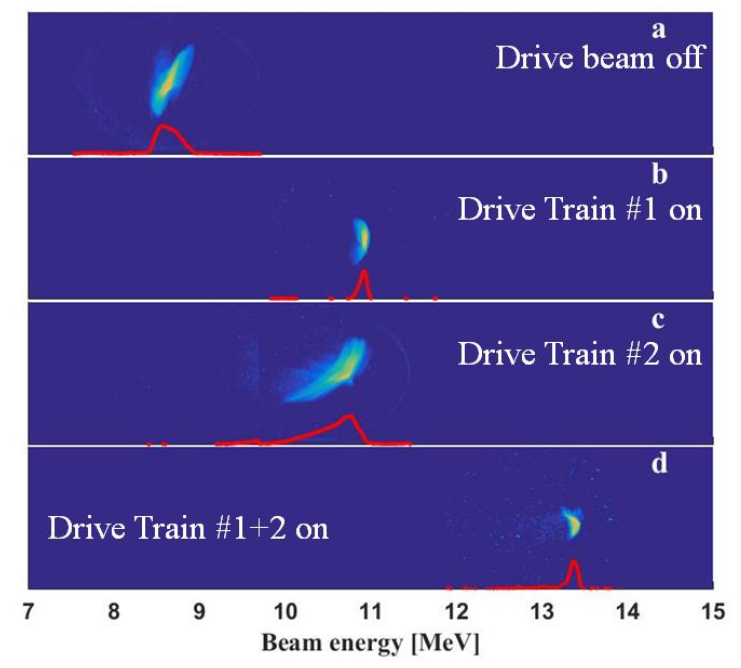
\includegraphics[width=0.75\textwidth]{images/old_tba}
	\label{fig:old-tba}
	\caption{Measurements of the energy during simplified staging experiments, 
		figure courtesy of Gwanghui Ha at AWA.
		Drive Train 1 refers to the stage one, and Drive Train 2 to stage 2. 
		Energy gain was observed in each stage independently.
		A larger energy gain was observed when both stages supplied RF to the witness beam line.}
\end{figure}
%%%%%%%%%%%%%%%%%%%%%%%%%%%%%%%%%%%%%%%%%%%%%%%%%%%%%%%%%%%%%%%%%%%%%%%%%%%%%%%%%%%%%%%%%%%%




\Section{Modifications to Reach Fully Staged TBA} \label{sec:requirements}

In order to design and test the desired beam line, three technologies 
new to the AWA were investigated. These include a kicker, septum magnets, 
and massively parallel optimization algorithms.


\lsnote{{\it Not sure if this section should be here, or later, more toward end of chapter.  This section is probably where you should have the overview of simple staging versus full staging, and a summary of what was required to go to full staging.  The title of the section should also be changed, maybe `Fully staged two beam acceleration'?  Probably need another (or repeated) figure here.}}
% An example for enumerate
\begin{enumerate}
        \item Kicker Design
        \item Septum Design
        \item Optimization
\end{enumerate}

%%%%%%%%%%%%%%%%%%%%%%%%%%%%%%%%%%%%%%%%%%%%%%%%%%%%%%%%%%%%%%%%%%%%%%%%%%%%%%%%%%%%%%%%%%%%
%%%%%%%%%%%%%%%%%%%%%%%%%%%%%%%%%%%%%%%%%%%%%%%%%%%%%%%%%%%%%%%%%%%%%%%%%%%%%%%%%%%%%%%%%%%%




\Section{Thesis Outline}

The rest of the thesis details work done at AWA.
Chapter 2 covers experimental measurements and preparations for TBA.
These include RF measurements and beam diagnostics (energy, beam size, and bunch length measurements).
Chapter 3 discusses simulation work done to model the drive line at AWA.
This includes optimization work.
Chapter 4 covers kicker and beam line optics design for fully staged TBA.

